\documentclass[aspectratio=169, french]{beamer}
\usepackage{fontspec}
\usepackage[french]{babel}
\usefonttheme[onlymath]{serif}
\usepackage{amsmath,amssymb,amsthm}
\usepackage{arydshln,mathtools}
\usepackage{bm}
\usepackage{color}
\definecolor{theme}{RGB}{0,73,114}
\usepackage{multicol}
%\usepackage[caption=false]{subfig}
\usepackage{subcaption}

\usepackage{comment}

\usepackage{graphicx}
\usepackage{diffcoeff}
\usepackage{dsfont}
\usepackage{mathrsfs}
\usepackage[most]{tcolorbox}

\usepackage{xspace}
\usepackage{appendixnumberbeamer}


\usepackage{media9}
\usepackage[backend=bibtex,style=verbose,doi=false,isbn=false,url=false,eprint=false,autocite=footnote]{biblatex}

\addtobeamertemplate{footnote}{\vspace{-6pt}\advance\hsize-0.5cm}{\vspace{6pt}}
\makeatletter
% Alternative A: footnote rule
\renewcommand*{\footnoterule}{\kern -3pt \hrule \@width 2in \kern 8.6pt}
% Alternative B: no footnote rule
% \renewcommand*{\footnoterule}{\kern 6pt}
\makeatother

\graphicspath{{./images/}}

\bibliography{biblio_pres}

\renewcommand\bibfont{\scriptsize}

% Remove navigation bar
\setbeamertemplate{navigation symbols}{}

\setbeamertemplate{blocks}[rounded][shadow]

\setbeamercolor{block body alerted}{bg=alerted text.fg!10}
\setbeamercolor{block title alerted}{bg=alerted text.fg!20}
\setbeamercolor{block body}{bg=structure!10}
\setbeamercolor{block title}{bg=structure!20}
\setbeamercolor{block body example}{bg=green!10}
\setbeamercolor{block title example}{bg=green!20}

\graphicspath{{./images/}}

\newif\iftocsub
\tocsubtrue
\AtBeginSection[] {
	\begin{frame}[noframenumbering]{Outline}
		\tableofcontents[sectionstyle=show/shaded, subsectionstyle=show/show/hide]
	\end{frame}
	\tocsubfalse
}
\AtBeginSubsection[] {
	\iftocsub
	\begin{frame}[noframenumbering]{Outline}
		\tableofcontents[currentsubsection, sectionstyle=show/shaded, subsectionstyle=show/shaded/hide]
	\end{frame}
	\fi
	\tocsubtrue
}

\newcommand{\beginbackup}{
	\newcounter{framenumbervorappendix}
	\setcounter{framenumbervorappendix}{\value{framenumber}}
}
\newcommand{\backupend}{
	\addtocounter{framenumbervorappendix}{-\value{framenumber}}
	\addtocounter{framenumber}{\value{framenumbervorappendix}} 
}


\begin{document}
	
	
\begin{frame}[plain]
	
	%%%%%%%% Title slide details %%%%%%%%%%%%%%


% Background Image
\newcommand{\myBackground}
{
    
\includegraphics[height=1.02\paperheight,page=9]{beamerthemeutresources}
}

% Title
\newcommand{\myTitle}
{
Projet d'intégration pour le poste
}

% Subtitle
\newcommand{\mySubTitle}
{
\textit{Enseignant-Chercheur en Méthodes Mathématiques pour le Calcul Scientifique}
}

% Author
\newcommand{\myAuthor}   
{
    Andrea Brugnoli
}

% Affiliation
\newcommand{\myAffiliate}
{
  
}

% Presentation Date
\newcommand{\myDate}   
{
    11 Avril 2022
}

% Logo
\newcommand{\myLogo}   
{
    
\includegraphics[width=3cm]{Logo.png}
}
%%%%%%%%%%%%%%%%%%%%%%%%%%%%%%%%%%%%


%%%%%%%%%% Title slide code %%%%%%%%%%%
\begin{tikzpicture}[remember picture,overlay]

% Background color

\fill[white] (current page.south west) rectangle (current page.north east);
% Background image
\node[above right,inner sep=0pt] at (current page.south west)
    {
        \myBackground
    };
    
% Title & Subtitle
\node
[
    above=0.5cm,
    align=center,
    draw=black!50,
    % rounded corners,
    double,
    double distance=0.1cm,
    double=blue!10,
    fill=theme!10,
    inner xsep=15pt,
    inner ysep=10pt, 
    minimum width=0.85\textwidth,
    text width=0.85\textwidth
] (title) at (current page.center)
{
    \LARGE \myTitle  \\[5pt]
    \small \mySubTitle
};

% Author 
\node[ below=0.5cm] (author) at (title.south){\myAuthor};

% Author 
\node[ below=0.25cm ](affiliate) at (author.south){\small \myAffiliate};

% Date
\node[below=0.25] (date) at (affiliate.south){\large \myDate};

% Logo
\node
[
    below =0.25cm
] at (date.south)
{
    \myLogo
};

\end{tikzpicture}
	
\end{frame}

	
	
\begin{frame}{Aperçu}
		
		\tableofcontents
		
\end{frame}
	
	\section{Enjeux du poste}
	
	\begin{frame}{La simulation numérique au service de l'ingénierie}
		
		\begin{columns}
			\begin{column}{.45\textwidth}
			\begin{figure}
				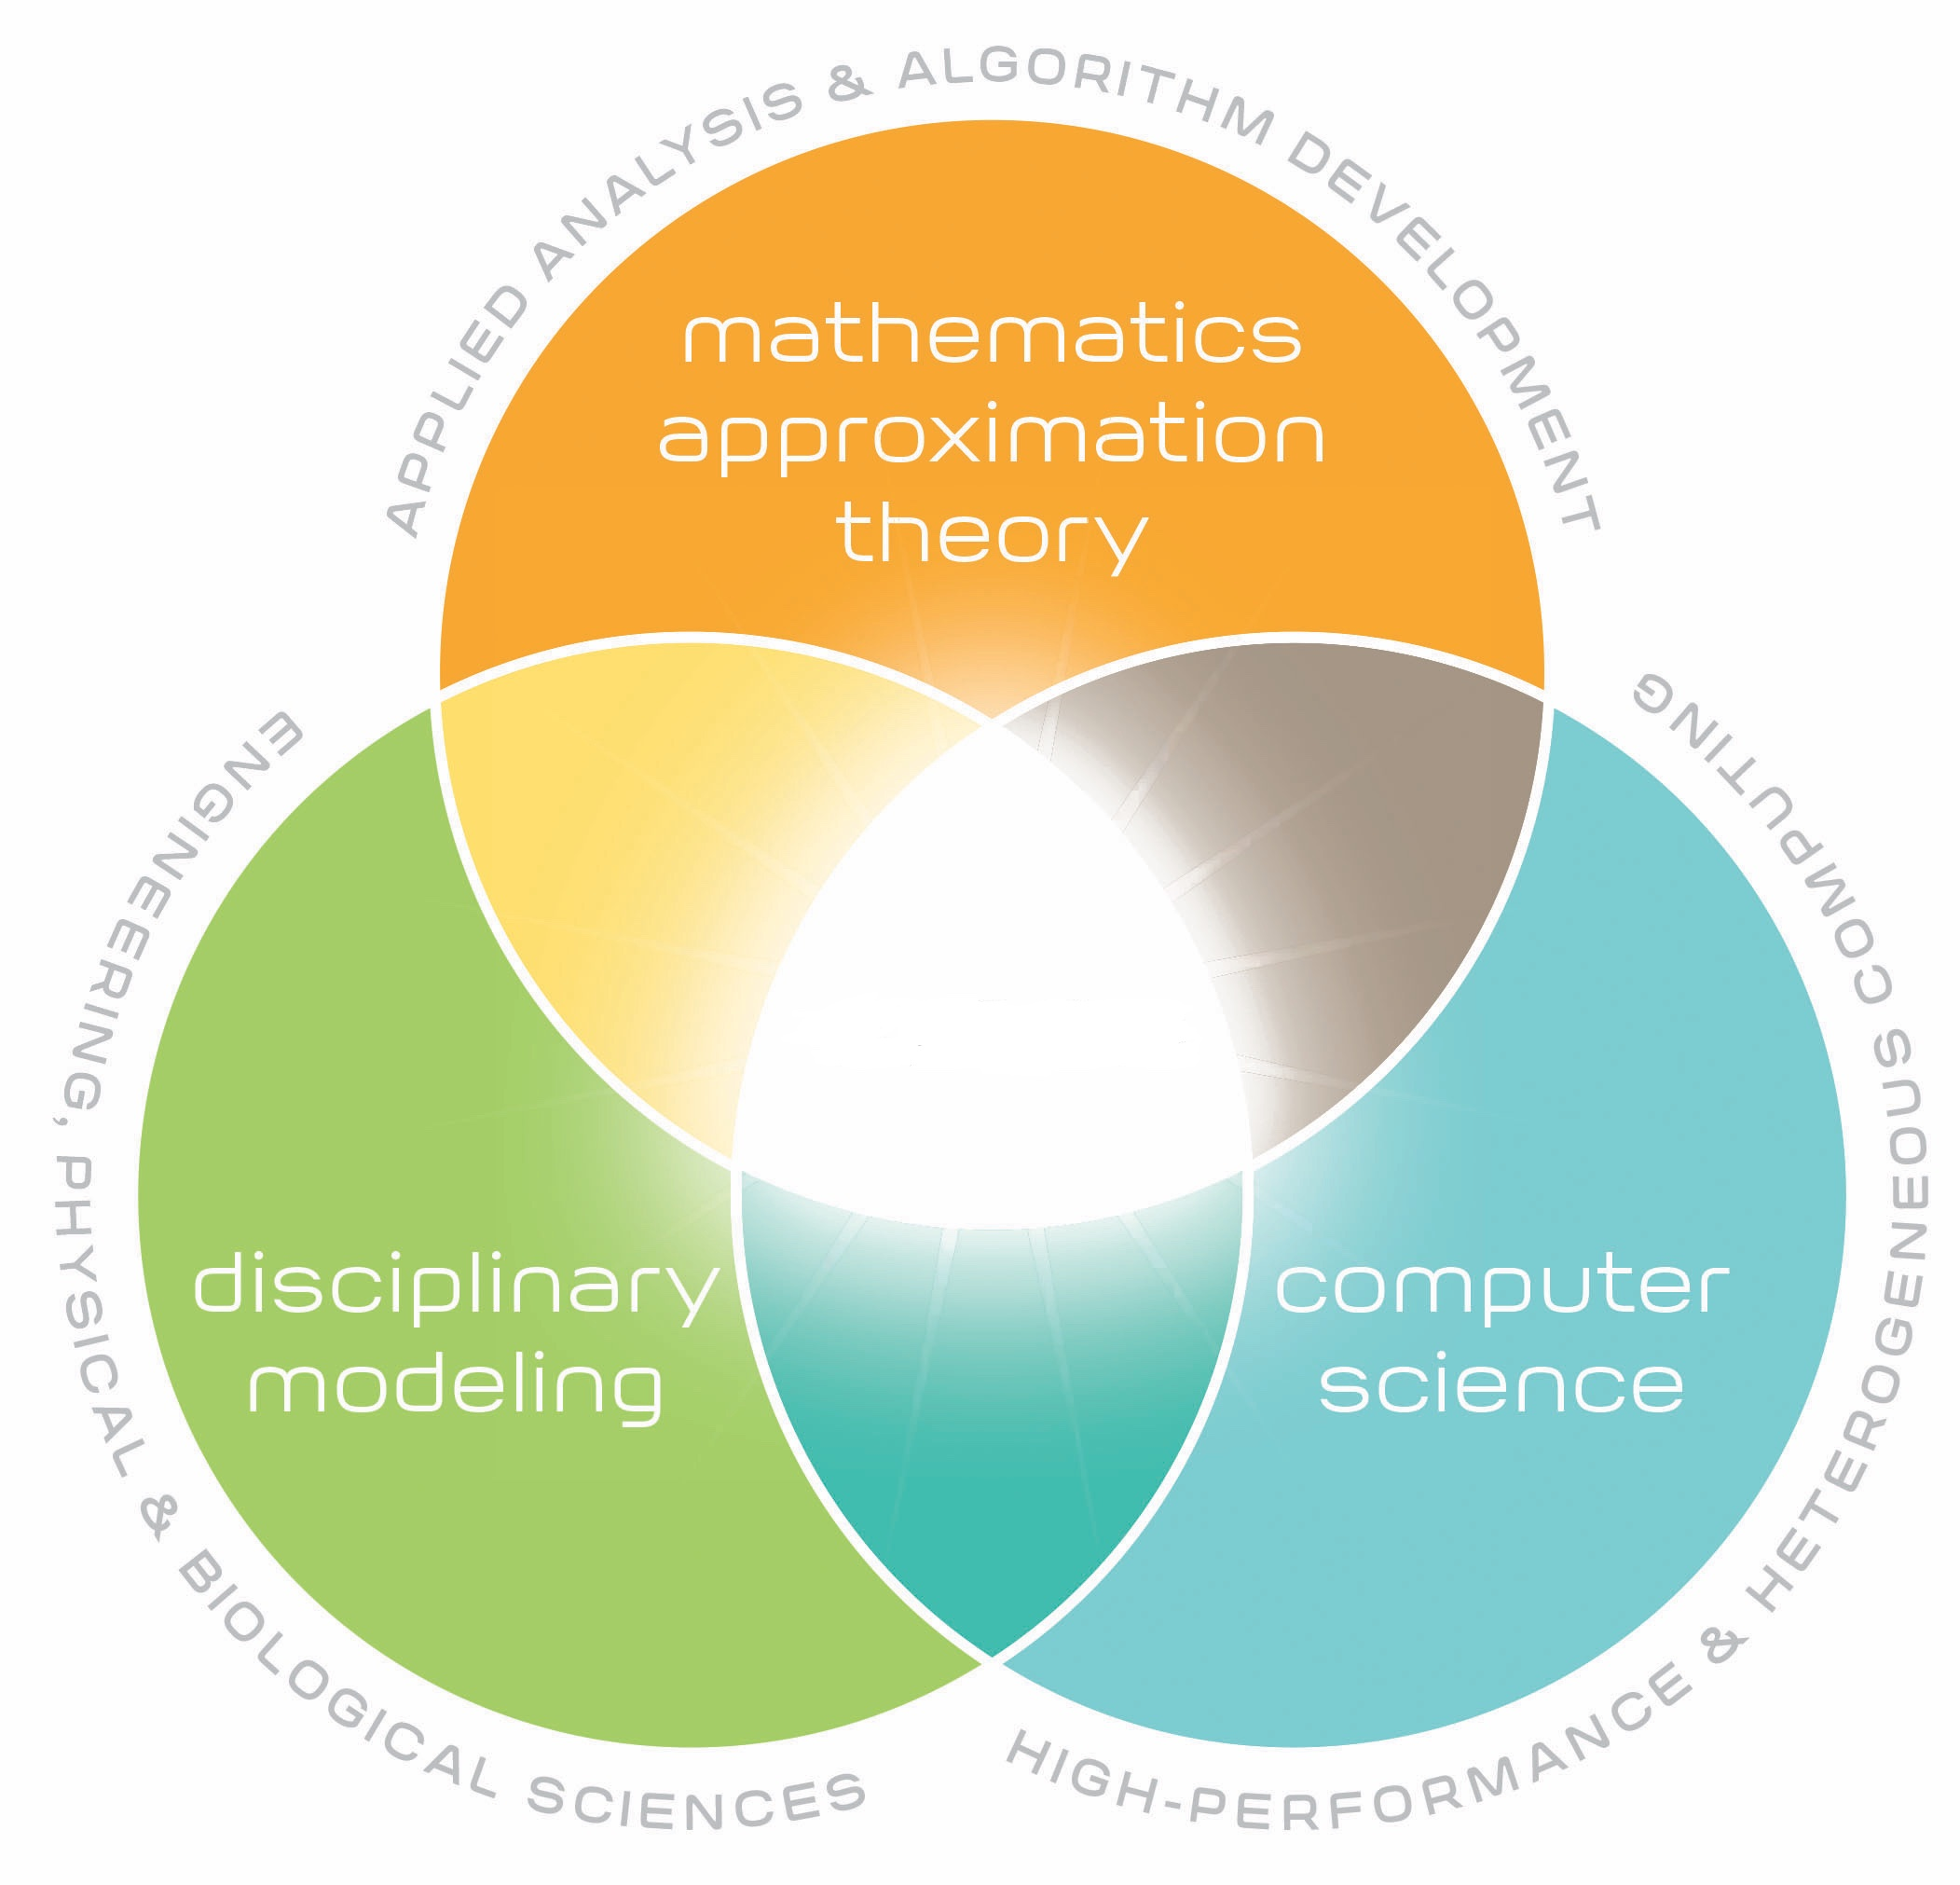
\includegraphics[width=.9\textwidth]{cse.jpg}
				\caption{\href{https://www.uio.no/english/studies/programmes/computational-science-master/why-choose/}{https://www.uio.no}}
			\end{figure}	
			\end{column}
			\begin{column}{.5\textwidth}
			Il s'agit d'une discipline multidisciplinaire, à l'intersection de\footnotemark :
			\begin{itemize}
				\item mathématiques appliquées (analyse numérique, discrétisation des EDP, optimisation);
				\item informatique et développement logiciel;
				\item modélisation physique.
			\end{itemize}
			
			\end{column}
		\end{columns}	
		\footcitetext{ulrich2018cse}
	\end{frame}

\begin{frame}{Activités d'enseignement prévues pour le poste}
	L'offre de formation ISAE-Supaero prévoit plusieurs cours pour cette discipline.\\
	\vspace{.5cm}
\textbf{Formation ingénieur (FISE)}:
\begin{itemize}
\item 1A : Méthodes numériques EDO et EDP 1D (différences finies, éléments finis).
\item 2A : Équations aux dérivées partielles - Théorie et simulations numériques.
\item 3A : Domaine SXS 
\begin{itemize}
	\item[--] Méthodes numériques pour la mécanique et la dynamique des fluides (éléments finis classiques et mixtes, volumes finis);
	\item[--] Calcul Haute performance (HPC));
\end{itemize}
\end{itemize}
\vspace{.5cm}
\textbf{Formation Mastère international MAE} :  EDP et calcul scientifique (en anglais).\\
\vspace{.5cm}
\textbf{Formation par Apprentissage (FISA)} : donner aux professionnels et apprentis les instruments nécessaires pour comprendre les logiciels des simulations.
	
\end{frame}

\begin{frame}{Supervision projets et Création de partenariats}	
Les partenariats industriels sont fondamentaux pour les PIR en 2A, les PIE du domaine SXS, et également les Stages de Fin Études.


\begin{columns}
	\begin{column}{.5\textwidth}
	Partenariats industriels : 
	\begin{itemize}
		\item CEA : simulation multiphysique.
		\item CERFACS : CFD et assimilation des données. 
		\item AIRBUS : aéroélasticité et mécanique.
		\item THALES : électromagnétisme, thermoélasticité.
	\end{itemize}
	\end{column}
	\begin{column}{.43\textwidth}
	\begin{figure}
		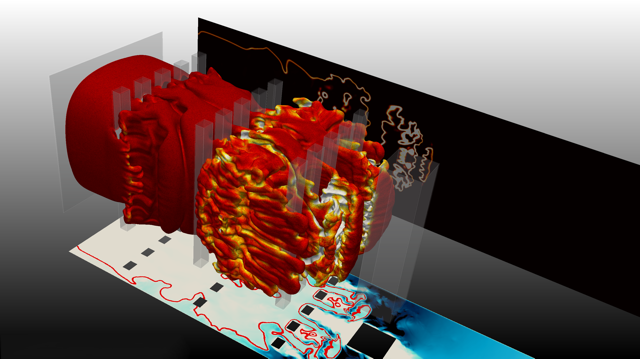
\includegraphics[width=1\textwidth]{image_CERFACS.png}
		\caption{\href{https://cerfacs.fr/logiciels-de-simulation-pour-la-mecanique-des-fluides/}{https://cerfacs.fr}}
	\end{figure}	
	\end{column}
\end{columns}
	
\end{frame}

\section{Projet d'intégration}

\begin{frame}{Analyse numérique et discrétisation des EDP}
	\begin{block}{Discrétisation structurée de modèles physiques pour l'ingénierie}
		Développement des activités de recherche liées à la modélisation et discrétisation structurées des EDP (port-)Hamiltoniennes.
	\end{block}

\begin{columns}		
	\begin{column}{.3\textwidth}
		\includemedia[
		label=vidPlateRod,
		addresource=/home/andrea/Videos/CandidatureISAE/KirchhRod.mp4,
		activate=pageopen, 
		deactivate=onclick,
		width=5cm, height=5cm,
		flashvars={
			source=/home/andrea/Videos/CandidatureISAE/KirchhRod.mp4
			&%
			autoPlay=true&%
			loop=true%
		}
		]{}{VPlayer.swf}
		%\mediabutton[
		%mediacommand=vidPlateRod:playPause
		%]{\fbox{Play/Pause}}
		2D plaque interconnectée
	\end{column}
	\begin{column}{.3\textwidth}
		\includemedia[
		label=vidTG2D,
		addresource=/home/andrea/Videos/CandidatureISAE/vorticityTG2D.mp4,
		activate=pageopen, 
		deactivate=onclick,
		width=5cm, height=5cm,
		flashvars={
			source=/home/andrea/Videos/CandidatureISAE/vorticityTG2D.mp4&%
			autoPlay=true&%
			loop=true%
		}
		]{}{VPlayer.swf}
		%\mediabutton[
		%mediacommand=vidTG2D:playPause
		%]{\fbox{Play/Pause}}
		2D Hydrodynamique
	\end{column}
	\begin{column}{.3\textwidth}
		\includemedia[
		label=vidMaxwell3D,
		addresource=/home/andrea/Videos/CandidatureISAE/MaxwellE13D.mp4,
		activate=pageopen, 
		deactivate=onclick,
		width=5cm, height=5cm,
		flashvars={
			source=/home/andrea/Videos/CandidatureISAE/MaxwellE13D.mp4
			&%
			autoPlay=true&%
			loop=true%
		}
		]{}{VPlayer.swf}
		%\mediabutton[
		%mediacommand=vidMaxwell3D:playPause,
		%]{\fbox{Play/Pause}}
		3D Maxwell
	\end{column}
\end{columns}	
%\mediabutton[
%mediacommand=vidPlateRod:playPause,
%overface=\color{blue}{\fbox{\strut Play/Pause}},
%downface=\color{red}{\fbox{\strut Play/Pause}}
%]{\fbox{\strut Play/Pause}}

%\mediabutton[
%mediacommand=vidPlateRod:setSource [(KirchhRod.mp4)]
%]{\fbox{\strut KirchhRod.mp4}}

\end{frame}




\begin{frame}{Agenda de recherche}
	
	\begin{block}{Thématiques de recherche}
		\begin{itemize}
			\item Analyse numérique des schémas.
			\item Lien entre géométrie et discrétisation : \textit{les éléments finis en calcul extérieur}.
			\item Stratégies pour le gain en performance : maillage adaptatif, solveurs et preconditionneurs, parallélisation du code et calcul haute performance. 
			\item Lien vers les applications : mécanique, dynamique des fluides, électromagnétisme, \textit{intelligence artificielle} et compression de données.
		\end{itemize}

		
	\end{block}
	
	
	\begin{block}{Développement logiciel}
		\begin{itemize}
			\item Développement d'un code de calcul pour la multiphysique (SCRIMP).
			\item Création d'un gitlab commun de travail, pour les doctorants, les stagiaires mais également pour le BE et TP des cours liés à la modélisation.
		\end{itemize}	
		
	\end{block}
	
\end{frame}


\begin{frame}{Transversalité au sein du DISC}
	L'\textbf{intelligence artificielle} offre des outils essentiels pour la compression de données issus des schémas de discrétisation.
	
	\begin{figure}[t]
		\begin{subfigure}[t]{0.48\textwidth}
			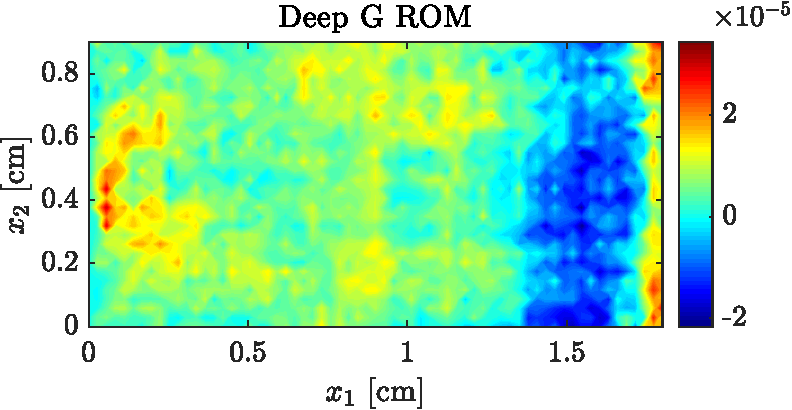
\includegraphics[width=\columnwidth]{DGROM_T_param1.pdf} 
			\caption*{Modèle réduit avec réseaux des neurones.}
		\end{subfigure}\hfill
		\begin{subfigure}[t]{0.48\textwidth}
			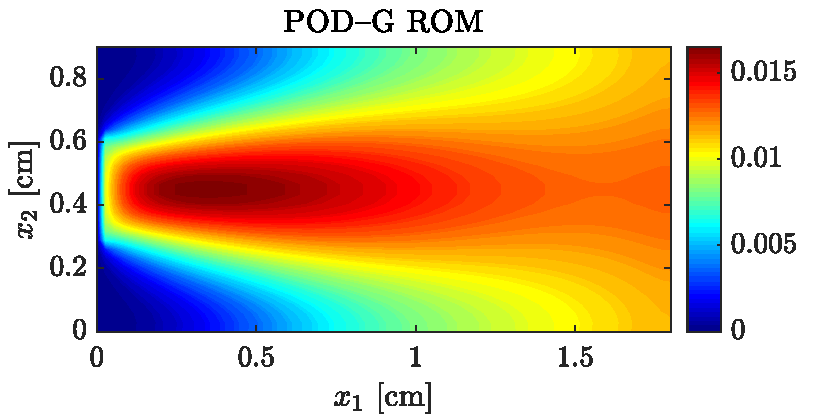
\includegraphics[width=\columnwidth]{GROM_T_param1.pdf}%
			\caption*{Modèle réduit avec la méthode linéaire POD.}
			\label{fig:POD_ROM}
		\end{subfigure}
		\caption*{Erreur des modèles réduits sur le champ de température pour un problème de convection-diffusion-réaction (Reproduit avec permission de \cite{lee2020}).}%
		\label{fig:deepROM}%
	\end{figure}
\end{frame}



\begin{frame}{Transversalité au sein de l'ISAE}
\begin{itemize}
	\item DMSM : mécanique structurelle et optimisation topologique. 
	\item DCAS : pour la réduction des modèles et le contrôle automatique.
	\item DAEP : dynamique des fluides.
\end{itemize}
\begin{figure}[t]
	\begin{subfigure}{0.45\textwidth}
		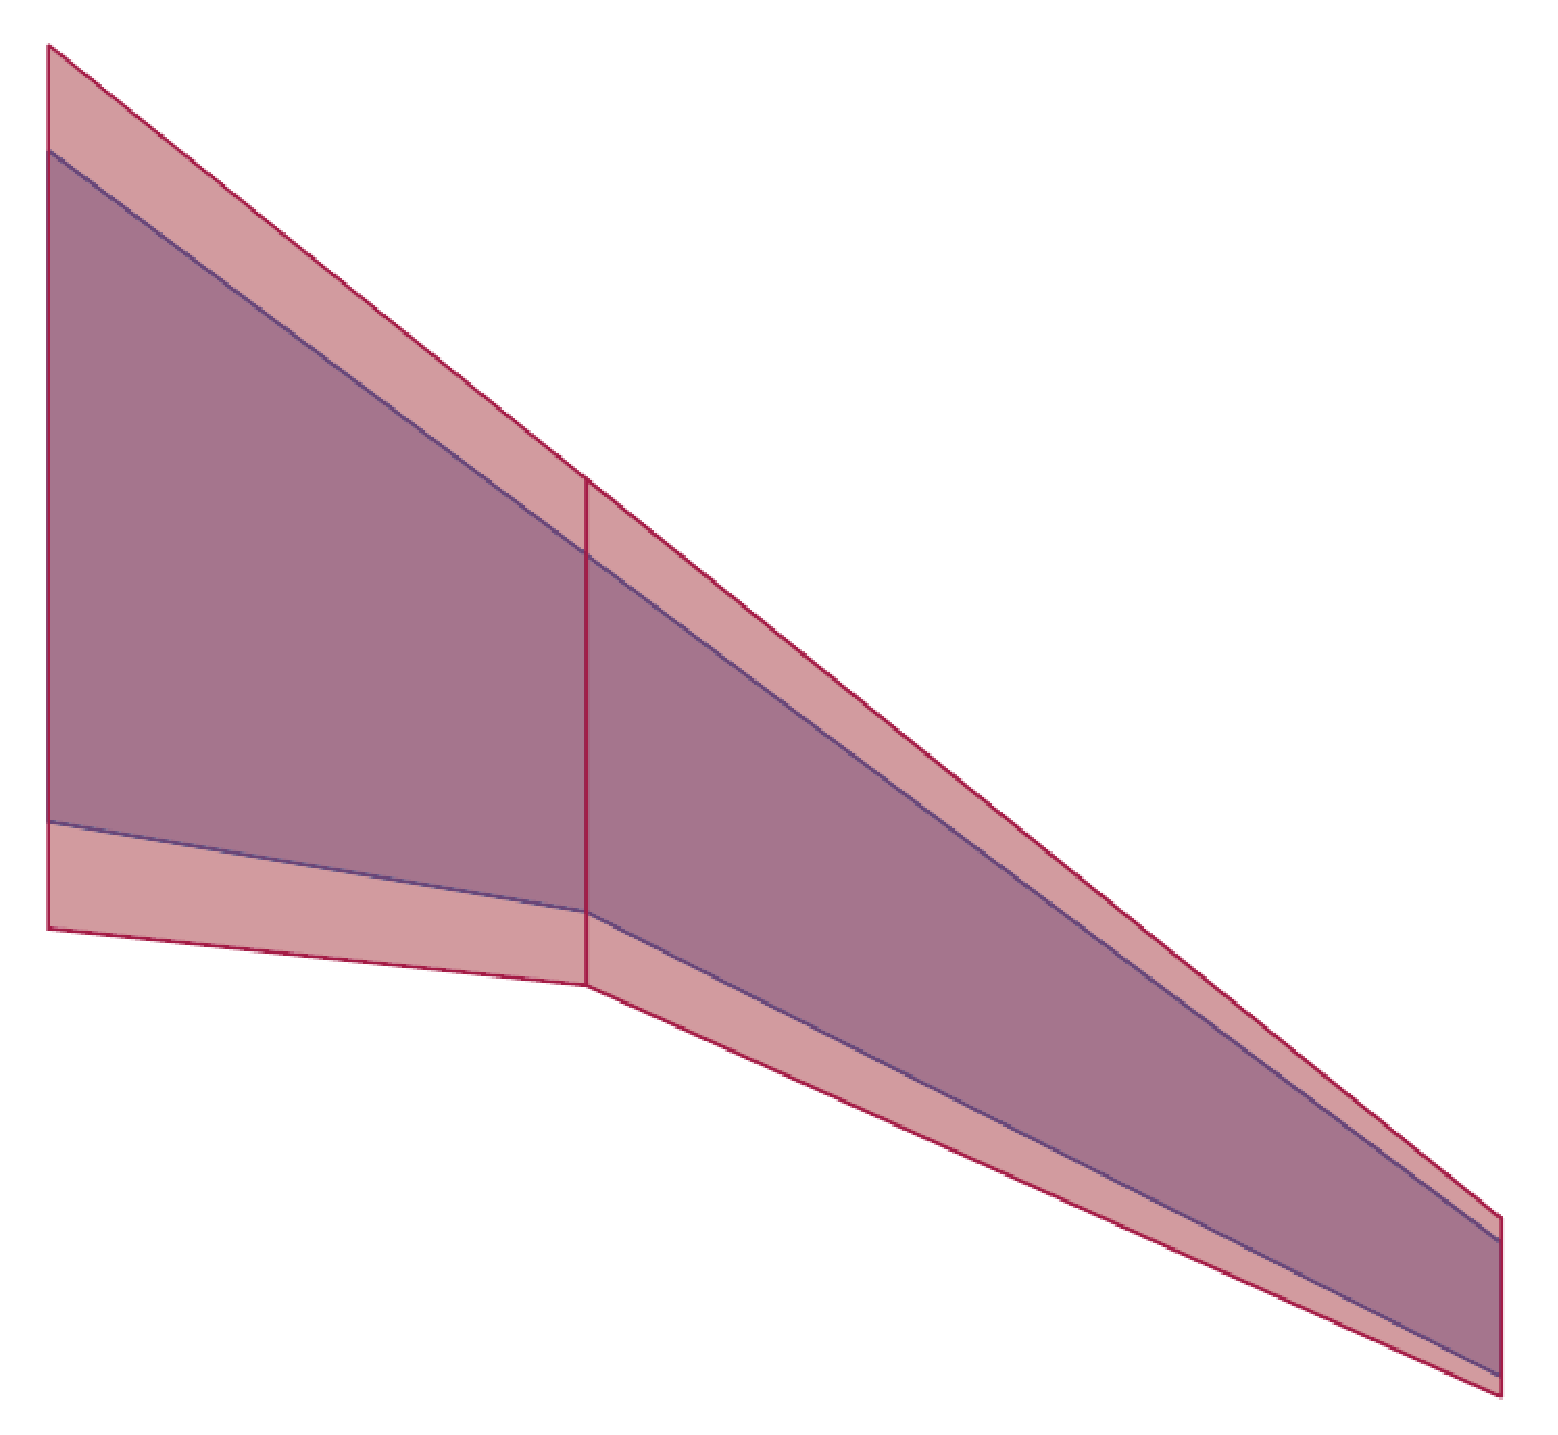
\includegraphics[height=.45\textheight]{MDO_wing.pdf}%
		\caption*{\textbf{Optimisation multidisciplinaire d'une aile} (\cite{masColomer2021mdo}). }
	\end{subfigure}\hfill
	\begin{subfigure}{0.5\textwidth}
		\includegraphics[height=.45\textheight]{Codesign_satellite.pdf} 
		\caption*{\textbf{Co-design contrôle/structure pour un satellite} (\cite{finozzi2022sub}).}
	\end{subfigure}
\end{figure}

\end{frame}


\begin{frame}{Modules électifs à proposer à moyen terme}
J'aimerais proposer des cours entre le calcul scientifique et les systèmes dynamiques :
\begin{itemize}
	\item Modélisation et discrétisation symplectique des structures flexibles complexes (intégration et continuation du module PFEM4PHS).
	\item Éléments de Géométrie différentielle pour la modélisation physique : du continu au discret.
\end{itemize}
\end{frame}

\begin{frame}{Collaborations}
\begin{figure}[t]
	\begin{subfigure}{0.5\textwidth}
		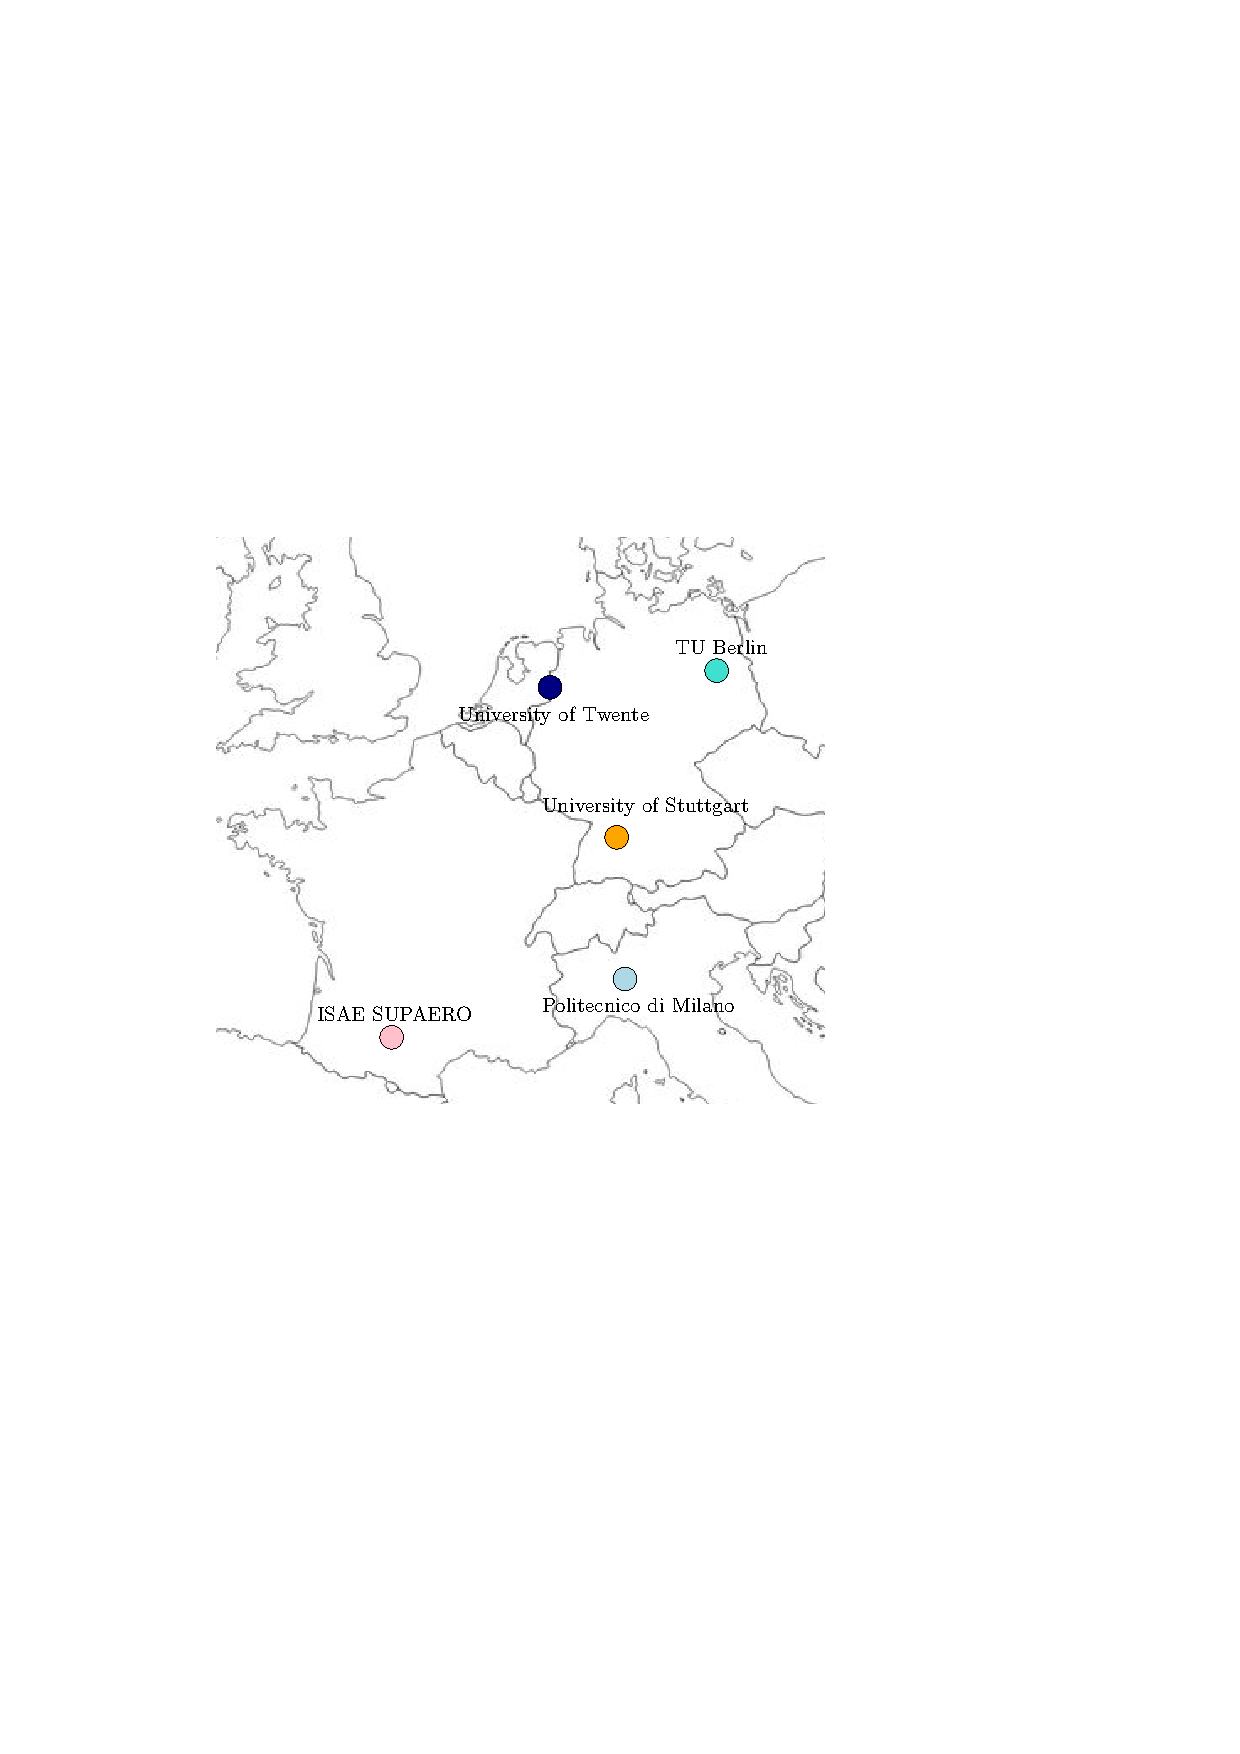
\includegraphics[width=.95\textwidth]{mappe_reseau_europe.pdf}%
	\end{subfigure}\hfill
	\begin{subfigure}{0.4\textwidth}
		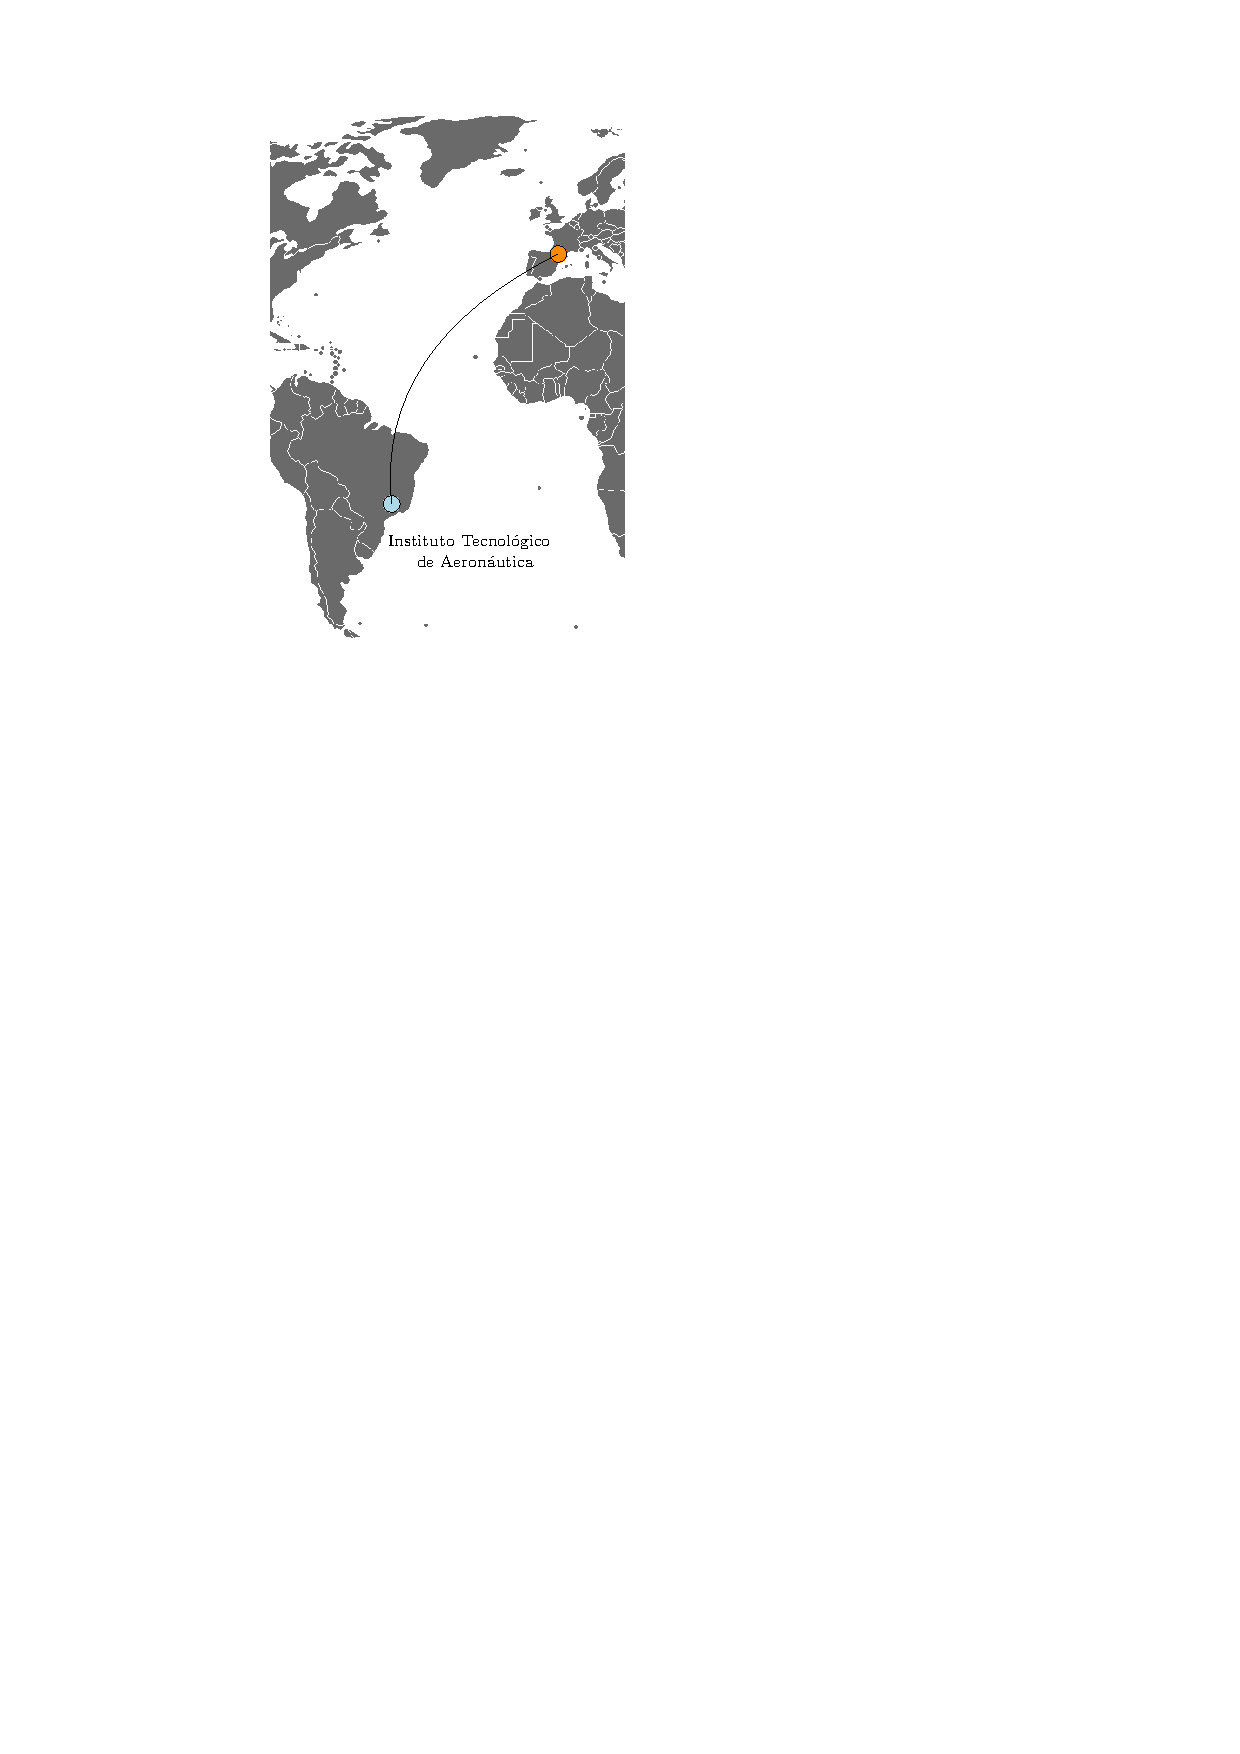
\includegraphics[width=.9\textwidth]{mappe_reseau_world.pdf} 
	\end{subfigure}
\end{figure}
\end{frame}

\begin{comment}
\begin{frame}[allowframebreaks]{Références}
\cite{brugnoli2019ammkir}\\
\cite{brugnoli2019ammkir}

\end{frame}
\end{comment}

	



\end{document}